\section{Durchführung}
\label{sec:Durchführung}


\subsection{Anpassung der Schwingkreise}
\begin{minipage}{0.5\textwidth}
    Zuerst muss der anpassbare Schwingkreis an die Resonanzfrequenz des Referenzschwingkreises angepasst werden, indem dort die Kapazität variiert wird.
    Also sucht man zuerst die Resonanzfrequenz des Referenzschwingkreises.
    Dafür nutzt man die in der Abbildung dargestellte Schaltung und probiert mit den Frequenzen so lange herum,
    bis die \textit{Lissajous-Figur} eine Gerade darstellt. Dies kann man am  Oszilloskop visuell darstellen.
    Hat man die Resonanzfrequenz gefunden, sind nun Spannung und Strom in Phase.
    Hat man diese gefunden, kann man den anderen Schwingkreis passend einstellen.
\end{minipage}
\begin{minipage}{0.5\textwidth}
    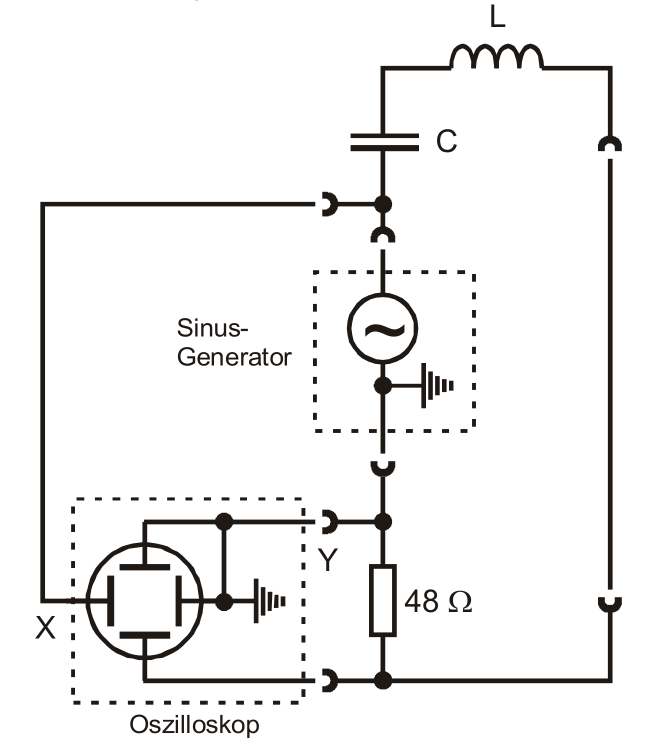
\includegraphics[width=\textwidth]{pictures/messschaltung.png}
\end{minipage}

\subsection{Messung}
\subsubsection*{Messung der Schwebungsfrequenz}
\begin{minipage}{0.3\textwidth}
    Nun möchten wir die nebenstehende Schaltung mit einem Rechteckspuls anregen.
    Durch die Widerstände von $R = 48 \Omega$ wird sich ein Spannungsabfall ergeben.
    Die Stromänderung möchjten wir am Oszilloskop visualisieren und dort auch die Schwebung beobachten.
    Jetzt werden die Maxima der Schwingung innerhalb einer Periode gezählt.
\end{minipage}
\begin{minipage}{0.7\textwidth}
    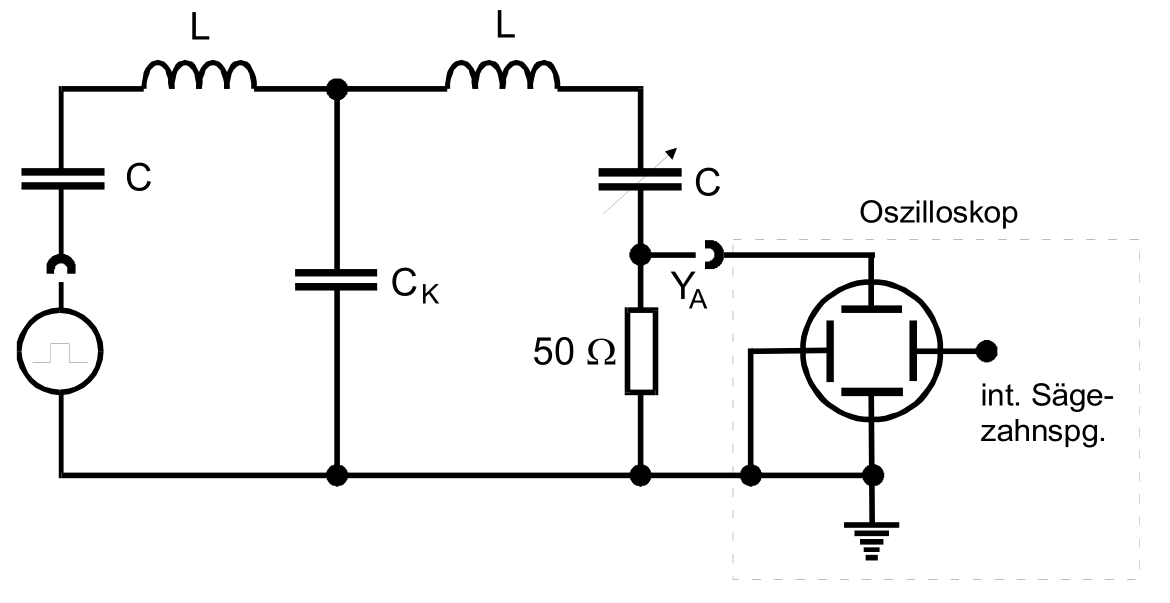
\includegraphics[width=\textwidth]{pictures/schwebeschaltung.png}
\end{minipage}

Damit lässt sich schließlich das Verhältnis der Schwebungsfrequenz und der Schwingungsfrequenz bestimmen.
Dieser Prozess wird für mehrere Kapazitäten durchgeführt.
Dabei sind Kapazitäten zwischen $C_{\text{min}} 2 nF$ und $C_{\text{max}} 12 nF$ möglich.

\subsubsection*{Fundamentalschwingungen}
Jetzt werden die Frequenzen $\nu^{-}$ und $\nu^{+}$ der \textit{Fundamentalschwingungen} in 
Abhängigkeit der Koppelkapazität $C_{K}$ gemessen.
Dafür wird die Anregung wieder auf eine Sinusanregung gestellt.
Zusätzlich wird die Generatorspannung als x-Ablenkung benutzt.
Nun sucht man wie zu Beginn mithilfe der Lissajous-Figuren die Frequenzen, bei denen die Phase 0 oder $\pi$ ist.
Dies wird für alle kapazitäten $C_{k}$ durchgeführt.

\subsubsection*{Verlauf der Ströme}

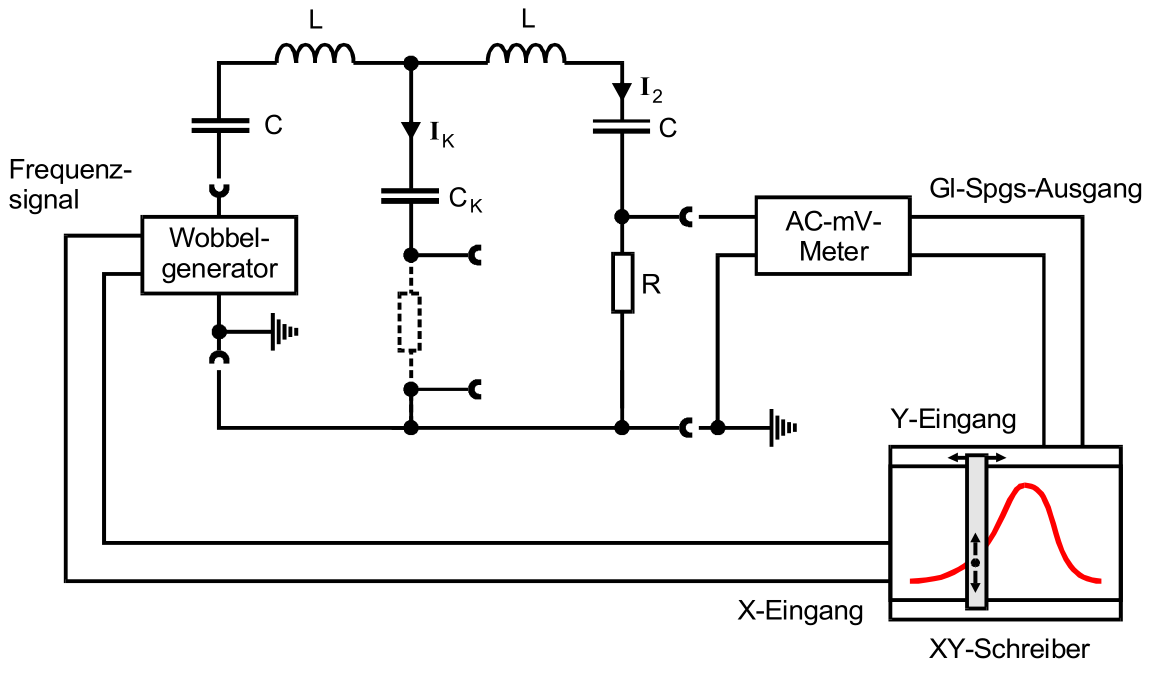
\includegraphics[width=\textwidth]{pictures/stromkurven.png}

Im folgenden werden die Verläufe der Ströme $I_{K}$ und $I_{2}$ in Abhängigkeit von der Frequenz
in der obigen Schaltung untersucht.
Dafür misst man den Spannungsabfall in den Widerständen mit einem AC-Breitband-Millivoltmeter.
Der sogenannte \textit{Wobbelgenerator} gibt neben der Wechselspannung auch noch ein Gleichspannungssignal.
Mit diesen Spannung lässt sich der XY-Schreiber ansteuern und  den Strom in Abhängigkeit der Frequenz visualisiert.
    